\documentclass[sigconf]{acmart}

\usepackage[english]{babel}
\usepackage{blindtext}
\usepackage{flushend}
%\hypersetup{colorlinks,linkcolor={blue},citecolor={blue},urlcolor={red}}  
%\usepackage{cite}
%\usepackage{color}
\hypersetup{pdfstartview=FitH,pdfpagelayout=SinglePage}
%\usepackage{footnote}
\setlength\paperheight {11in}
\setlength\paperwidth {8.5in}
\setlength{\textwidth}{7in}
\setlength{\textheight}{9.25in}
\setlength{\oddsidemargin}{-.25in}
\setlength{\evensidemargin}{-.25in}

\usepackage{booktabs} 

%\usepackage{forest}
\usepackage{varwidth}
\usepackage{enumitem}
\usepackage{float}
\usepackage{graphicx}
\usepackage{rotating}
\usepackage{caption}
%\usepackage[hang,small,labelfont=,textfont=]{caption}
\usepackage[font=scriptsize,format=plain,labelfont=bf,textfont=bf]{caption}
\usepackage{wrapfig}
%\setlength\intextsep{0pt}
\usepackage[font=footnotesize]{subcaption}
\usepackage{amsfonts}
\usepackage{multirow}
%\usepackage{multicol}
%\setlength{\columnsep}{20pt}
%\setlength{\columnseprule}{0.01pt}
\usepackage{listings}
\lstset{basicstyle=\ttfamily,
	breaklines=true}

%\setlength{\textwidth}{469pt}
\usepackage{mdwlist}
\usepackage{comment}
\usepackage{scrextend}
\usepackage[linesnumbered,ruled,vlined]{algorithm2e}
%\usepackage{verbatim}
\usepackage{fancyvrb}
%\usepackage[noend]{algorithm2e}
%\pagestyle{empty}
\SetKw{KwBy}{by}
%\usepackage{algorithmicx}
\usepackage{relsize}
\usepackage{tabularx}

\usepackage{bold-extra}
\usepackage{xcolor}
\usepackage[section]{placeins}
\usepackage{tablefootnote}
%\newcommand{\citeColored}[2]{{\hypersetup{citecolor=#1}\cite{‌​#2}}}
%\usepackage{xcolor}
%\usepackage[section]{placeins}
\usepackage[english]{babel}
%\usepackage{url}
\usepackage{hyperref}
\usepackage{fancyhdr} 
\fancyhf{}
\cfoot{\thepage}
\pagestyle{fancy} 
\newcommand\mycommfont[1]{\tiny\ttfamily\textcolor{blue}{#1}}
\SetCommentSty{mycommfont}
\newcommand{\smartparagraph}[1]{\vspace{.05in}\noindent{\bf #1}}
%
% All template tuning for space reasons goes here
%
%\usepackage{titling}
%\setlength{\droptitle}{-10em} 
\usepackage{mdwlist}
\usepackage{makecell}

\renewcommand\theadalign{cb}
\renewcommand\theadfont{\bfseries}
\renewcommand\theadgape{\Gape[4pt]}
\renewcommand\cellgape{\Gape[4pt]}
\newcommand{\ap}[1]{\textit{\textcolor{purple}{[Apoorv]: #1}}}
\newcommand{\kh}[1]{\textit{\textcolor{cyan}{[Kevin]: #1}}}
\renewcommand{\footnotesize}{\tiny}
%\settopmatter{printfolios=true}
% Copyright
%\setcopyright{none}
%\setcopyright{acmcopyright}
%\setcopyright{acmlicensed}
%\setcopyright{rightsretained}
%\setcopyright{usgov}
%\setcopyright{usgovmixed}
%\setcopyright{cagov}
%\setcopyright{cagovmixed}
\usepackage{cleveref}
%\makeatletter
%\ifcase \@ptsize \relax% 10pt
%\newcommand{\miniscule}{\@setfontsize\miniscule{4}{5}}% \tiny: 5/6
%\or% 11pt
%\newcommand{\miniscule}{\@setfontsize\miniscule{5}{6}}% \tiny: 6/7
%\or% 12pt
%\newcommand{\miniscule}{\@setfontsize\miniscule{5}{6}}% \tiny: 6/7
%\fi
%\makeatother
% You don't want to use \subparagraph
\crefformat{section}{\S#2#1#3} % see manual of cleveref, section 8.2.1
\crefformat{subsection}{\S#2#1#3}
\crefformat{subsubsection}{\S#2#1#3}


\begin{comment}
\let\stditemize\itemize
\let\endstditemize\enditemize
\let\itemize\undefined
\makecompactlist{itemize}{stditemize}
% Modify section headers
\usepackage{titlesec}

 % You don't want to use \subparagraph



% Paper dimension magic
\setlength{\paperheight}{11in}
\setlength{\paperwidth}{8.5in}
\setlength{\textwidth}{6.5in}
\setlength{\textheight}{9in}
\setlength{\oddsidemargin}{-.25in}
\setlength{\evensidemargin}{-.25in}

% Get the captions to not eat up all the space
%\setlength{\abovecaptionskip}{20pt}
%\setlength{\belowcaptionskip}{-3pt}
\setlength{\floatsep}{5pt}
\setlength{\textfloatsep}{9pt}
\setlength{\dbltextfloatsep}{3pt}
\setlength{\intextsep}{3pt}
\end{comment}
\sloppy

\floatsep 4pt plus 2pt minus 2pt       % Space between adjacent floats moved
% to top or bottom of text page.
\textfloatsep 5pt plus 2pt minus 4pt   % Space between main text and floats
% at top or bottom of page.
\intextsep 4pt plus 2pt minus 2pt      % Space between in-text figures and
% text.
\dblfloatsep 4pt plus 2pt minus 2pt    % Same as \floatsep for double-column
% figures in two-column mode.
\dbltextfloatsep 4pt plus 2pt minus 4pt% \textfloatsep for double-column
% Copyright
\renewcommand\footnotetextcopyrightpermission[1]{} % removes footnote with conference info
\setcopyright{none}
%\setcopyright{acmcopyright}
%\setcopyright{acmlicensed}
%\setcopyright{rightsretained}
%\setcopyright{usgov}
%\setcopyright{usgovmixed}
%\setcopyright{cagov}
%\setcopyright{cagovmixed}

\settopmatter{printacmref=false, printccs=false, printfolios=true}

% DOI
\acmDOI{}

% ISBN
\acmISBN{}

%Conference
%\acmConference[Submitted for review to SIGCOMM]{}
%\acmYear{2018}
%\copyrightyear{}

%% {} with no args suppresses printing of the price
\acmPrice{}
\newcommand{\system}{$\textsc{P4ML}$\xspace}
% Program Behaviour Description Language/Logic (PBDL)
\newcommand{\lang}{$\textsc{PBDL}$\xspace}
\begin{document}
\title{Reinforcement Learning for P4 Program Verification}

%\titlenote{Produces the permission block, and copyright information}
%\subtitle{Extended Abstract}

\author{Paper \# XXX, XXX pages}
% \author{Firstname Lastname}
% \authornote{Note}
% \orcid{1234-5678-9012}
% \affiliation{%
%   \institution{Affiliation}
%   \streetaddress{Address}
%   \city{City} 
%   \state{State} 
%   \postcode{Zipcode}
% }
% \email{email@domain.com}

% The default list of authors is too long for headers}
\renewcommand{\shortauthors}{X.et al.}
%\newcommand{\ap}[1]{\textit{\textcolor{purple}{[Apoorv]: #1}}}
\begin{abstract}
Everybody loves TCP. The paper body in this example
using the HotNets 2017 style file contains two copies
of the CFP text to show the correct format of a standard text page.

\end{abstract}

\maketitle

%\section{Introduction}
\Blindtext

\begin{figure}[tp]
\centering

\includegraphics{figures/mouse}
\caption{\blindtext}
\end{figure}

\section{Related Work}
\blindtext

And we need some citation here\cite{Stoenescu:2018:DPP:3230543.3230548, Liu:2018:PPV:3230543.3230582, Freire:2018:UBP:3185467.3185499, Neves:2018:VPP:3281411.3281421, Notzli:2018:PAT:3185467.3185497}

\Blindtext

\section{System Design}

\subsection{The First Layer}
\Blindtext

\subsection{The Second Layer}
\Blindtext

\section{Evaluation}
\Blindtext

\section{Conclusion}
\blindtext


%\begin{abstract}
%Everybody loves TCP. The paper body in this example
using the HotNets 2017 style file contains two copies
of the CFP text to show the correct format of a standard text page.

%\end{abstract}

\ap{In total: 4-5 plots, 3 figures, 1 code snippet, 1 table of rel. work, 14-15 valid references}
\section{Introduction}
\ap{2 Pages for: Introduction + Motivating Examples + Rel. work}

\ap{The architectural difference btw Bmv2 and Tofino. Processing pipeline, CP, etc.}

Motivation/ introduction:
\begin{itemize}
    \item Network verification is important as softwarization of the data plane is getting more and more attention in research as well as the industry
    \item because network outages are costly and small errors can lead to whole network outages
    \item existing verification approaches are not sufficient
    % should the next points with hint on why existing work is insufficient be here already? or is it better to fully move that to related work?
    \item existing approaches can already capture few kinds of bugs but are either based on symbolic execution, which is suffering from path explosion problem if the program is branchy
    \item and/or assume a lot of additional manual work to reflect expected program behaviour
    \item so these approaches are either lacking possibilities to also verify large or branchy programs but also require manual work even if the programs to be verified implement the same high level logic, e.g. layer 3 packet processing.
    \item Problem statement: Can the correctness of P4 programs be automatically verified?
    \item this paper aims at using radically different approaches changing the game of network verification and providing a solution to automatically verify P4 programs for a wide variety of common bugs in P4 programs.
    \item contributions: 
    \item implement reinforcement learning assisted fuzzing framework/ approach to automatically verify P4 programs overcoming several limitations of existing work.
    
\end{itemize}
\section{Motivating Examples}
\ap{draw clean diagrams in pdf using google presenation with scenarios just like in PAZZ which P4v, Vera, ASSERT etc cannot detect}

\begin{figure}[tp]
\centering
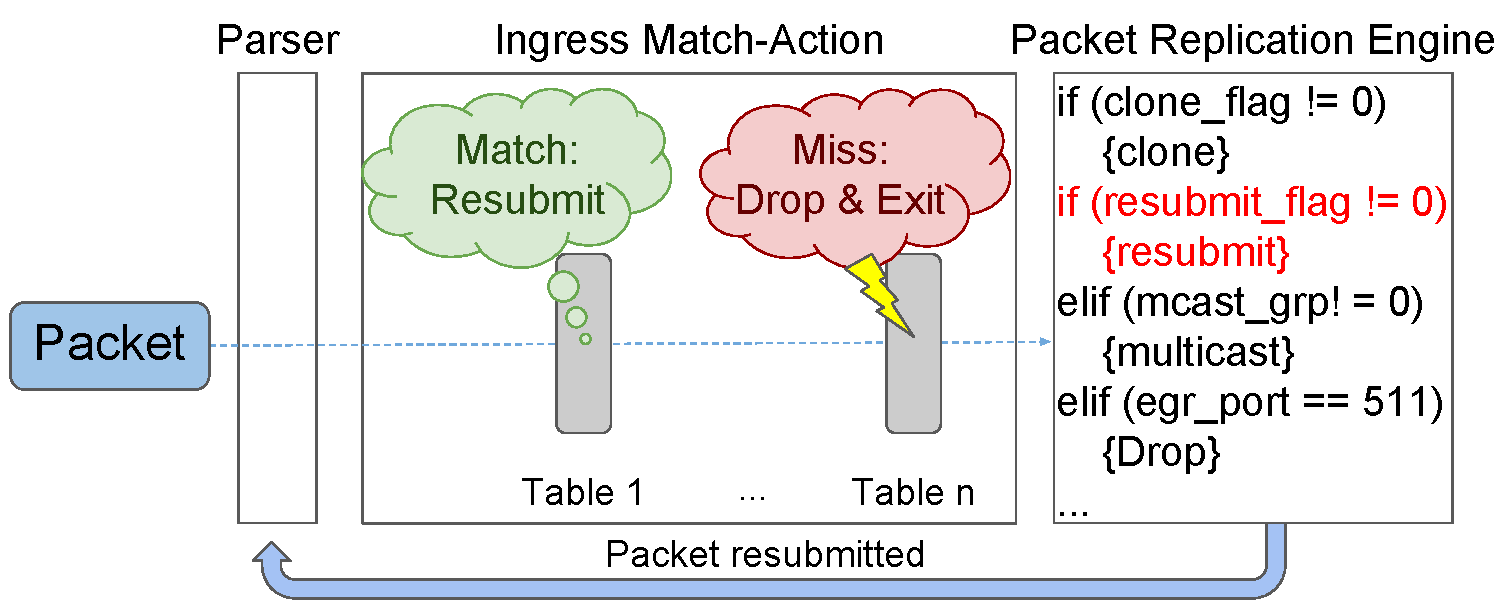
\includegraphics[width=\linewidth]{figures/scenario_v5.pdf}
\caption{Example of Target Specific Drop} %\ap{Font looks too small so make sure it is readable by naked eye. Use clker.com for free images which are not copyright}
\end{figure}
Example scenario:
\begin{itemize}
    \item After Packet traversed the parser it is processed in ingress processing
    \item during ingress processing tables are applied
    \item if e.g. a packet is matched in a table and as a result a resubmit action is executed, the resubmit flag for that packet will be set (part of the metadata)
    \item if in a later stage the packet is marked for drop and ingress processing is aborted, e.g. miss in ACL table, the packet reaches the packet replication engine (PRE).
    \item The architecture/target specific implementation defines what happens with such a packet. In Bmv2 with simple switch target (standard target from tutorials), the packet would be resubmitted even though the programmer would expect it to be dropped.(see figure)
\end{itemize}

Verification approaches and comparison (or should that be part of related work?) Or only introducing Fuzzing?
\begin{itemize}
    \item Fuzzing is ...
    \item types of fuzzing (White-box, grey-box, black-box, dumb, smart, generation based, mutation based, ...?)
    \item
\end{itemize}
quick intro on machine learning/ reinforcement learning
\begin{itemize}
    \item What is machine learning?
    \item taxonomy
    \item reinforcement learning
    \item Q learning
    \item deep Q learning
    \item usually used to let computers learn to play games (maybe ref. Google Deepmind papers as examples)
\end{itemize}


\section{Related Work}
\begin{itemize}
    \item why are existing approaches insufficient?
    \item symbolic execution drawbacks --> why is symbolic execution limited? --> only focuses on what code is there but not on problems that arise from unimplemented features. 
    \item manual assertion drawbacks
    \item one by one explanation of the existing work (Vera~\cite{Stoenescu:2018:DPP:3230543.3230548}, p4v~\cite{Liu:2018:PPV:3230543.3230582}, Assertion-based verification~\cite{Freire:2018:UBP:3185467.3185499}~\cite{Neves:2018:VPP:3281411.3281421},  p4pktgen~\cite{Notzli:2018:PAT:3185467.3185497}) and explaining what the drawbacks of each of the solutions are and what kind of bugs they can not detect, which we can detect.
    \item existing approaches can already capture several kinds of bugs but are either based on symbolic execution, which is suffering from path explosion problem if the program is branchy
    \item or assume a lot of additional manual assertions inside the code to reflect expected program behaviour
    \item or require the programmer to learn logic expression language and express the whole program behaviour using that logic
    \item so these approaches are either lacking possibilities to also verify large or branchy programs but also require manual work even if the programs to be verified implement the same high level logic, e.g. layer 3 packet processing.
\end{itemize}
\ap{Also include related works like Cocoon etc. cited in Vera, P4v, ASSERT-P4, P4Packetgen to make an exhaustive table of related work to compare to make it crystal clear what they don't do and we do, like $\times$, \checkmark}
\section{Methodology}
What is our verification approach?

\ap{Think about a simple language/constructs or utility, we provide to users for specifying properties that we would like to verify. That will have a better impact. }
\begin{itemize}
    \item explain the idea of combining mutation based fuzzing with the reinforcement learning:
    \item interpreting mutation based fuzzing as game to be able to apply reinforcement learning methods
    \item connect mutation based fuzzing as game for reinforcement learning, with verification through sending packets with mutated header values to test for/ trigger bugs by comparing the packet as it was sent to the ingress port of the switch with the resulting processed packet at egress of the switch and applying rules for checking e.g. protocol compliant processing.
    \item use this result as input for reward function, providing the feedback used to train the reinforcement learning model
\end{itemize}
\section{Implementation and Evaluation}
\ap{1 Page for: Implementation + Evaluation + Discussion}

\subsection{Implementation}
\begin{itemize}
    \item software architecture
    \item software modules developed
    \item frameworks \& tools used
\end{itemize}

\subsection{Evaluation}
\ap{For now, include handmade plots that we expect and also figures so that we have an idea of how much space we are left with?}

\begin{itemize}
    \item What are the metrics that should be evaluated?
    \item performance metrics: execution time, individual bug detection time?, how many bugs were detected?,
    \item metrics to evaluate the machine learning approach:
    \item cumulative reward over time (during training phase), to indicate the quality of the learning process
    \item ???
\end{itemize}
\section{Discussion}
\begin{itemize}
    \item overall results
    \item challenges
    \item limitations
    \item future work
\end{itemize}
\section{Conclusion}


\bibliographystyle{ACM-Reference-Format}
\bibliography{refs.bib}

\end{document}